% Chapter 3

\chapter{Research Methodology} % Main chapter title

\section{Introduction}
This section describes which research approach was chosen and why. Further, it elaborates, how the research approach is implemented and what work is done in the corresponding sections. 

\section{Research Design}
As research methodology experimental research was chosen. Experimental research typically focuses on systematically testing a hypothesis. It is often applied to research fields such as physics and chemistry but also psychology. In the this research project, the hypothesis to test is formulated as the thesis statement (see section \ref{thesisstatement}.\\
\\
Experimental research knows five process steps. These are:

\begin{itemize}
	\item Awareness of the Problem
	\item Design of Experiments
	\item Experiments
	\item Evaluation
	\item Conclusion
\end{itemize}

In the following, it is outlined what will be done in the different process steps and how it is going to help answering the research question and test the thesis statement. Figure \ref{Thesis Map} illustrates the different steps.

\begin{figure}[h]
	\centering
	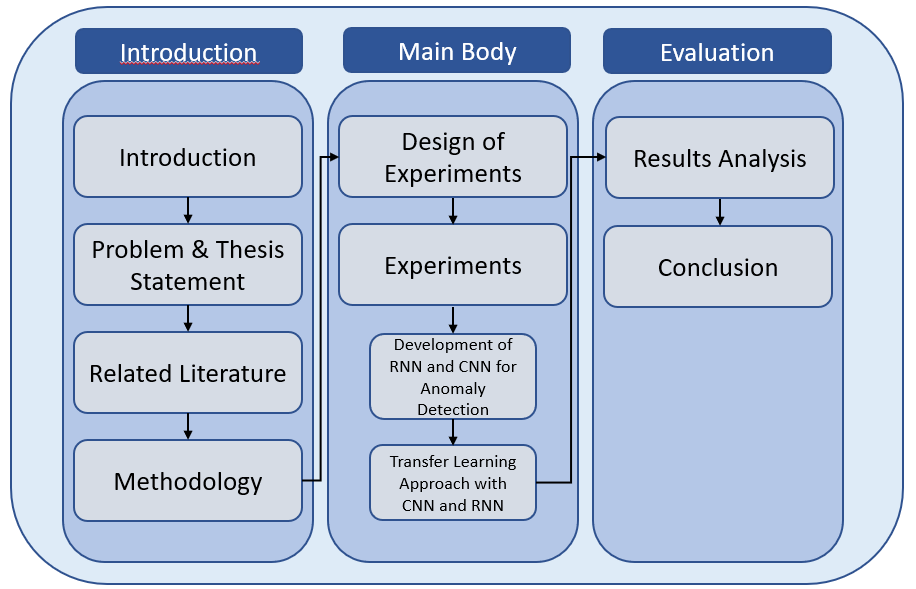
\includegraphics[scale=0.5]{Figures/Thesis Map}
	\decoRule
	\caption[Thesis Map]{Thesis Map \parencite{own}}
	\label{Thesis Map}
\end{figure}

\newpage
\subsection{Awareness of the Problem - Literature Review}
In this work, the literature review consists of two parts, background information presented in Section \ref{background} and the part Related Literature presented as Chapter \ref{relatedLiterature}. The reason for this split is to give insight on how neural networks and especially the derived architectures such as CNN and RNN work. A basic understanding of these two architectures is required to comprehend the problem and thesis statement presented in Sections \ref{Problem} and \ref{thesisstatement}. 

Further, the part Related Literature should deliver insights on how CNN and RNN are applied to detect anomalies. Where helpful, the publications investigated not only focus on detecting anomalies but also on related fields such as classification or prediction of time series. The investigated knowledge fields should serve as suggestions on how anomaly detection models can be set up. Next, the possibilities of transfer learning are examined. Since artificial intelligence experiences a boom in recent years, and neural networks are used more frequently, the possibilities offered by transfer learning will increase. Even more important, transfer learning is able to tackle one of the fundamental problems in anomaly detection. It enables to learn a performant model, even on a small data set. 

At last, to be able to answer the research question it is investigated how the different architectures, RNN and CNN, can be compared and what measures are important. 

\subsection{Experimental Design}
In this section, it is outlined how the experiments are designed. It is described how and why datasets are selected as well as which architecture principles are followed when designing the neural networks.

\subsubsection{Data Selection}
As described in Section \ref{anomalies}, there are different kinds of anomalies, which are more or less difficult to detect. Section \ref{Transferlearning} Transfer Learning further shows that the relationship of the source domain and target domain data set is of significant importance for the quality of the results. These two facts indicate that the data sets used for the experiments need to be carefully selected. In the Section Design of Experiments suitable data sets are proposed. At least, three different data sets are selected to conduct experiments. One of these data sets represents the source domain for transfer learning and another one the target domain. To learn the generic features necessary for transfer learning the data set used as source domain needs to consist of a large amount of data.

Further, the selected data sets have a direct impact on how the experiments have to be designed. Here the decision has to made, whether an unsupervised or supervised approach is applied. A supervised approach hereby requires a data set where the anomalies are labelled. In contrast, an unsupervised approach can investigate any time series data for anomalies but it is difficult to validate the achieved results. 

\subsubsection{Setup of Experiments}
In the Section Setup of Experiments the general setup of the experiments is elaborated. Chapter \ref{relatedLiterature} showed that there are various approaches on how to detect anomalies. Anomalies can either be directly classified by the neural network or detected via an anomaly threshold. This decision has to made based on the chosen data set, since only in a supervised approach a network can be designed to directly classify whether an anomaly is present. In Section \ref{SetupOfExperiments} a suitable method to answer the research questions is proposed. In addition, the advantages of the proposed setup, especially with an outlook on how the achieved results can be compared, are elucidated.   
Further, in Section \ref{SetupOfExperiments}, all global parameters are defined. Global paramters are parameters that need to be defined manually rather than learned, and are valid for all experiments. An example of such a global parameter could be the optimizer function and its corresponding parameters.

\subsection{Experiments}
Finally, in the Section Experiments the proposed experimental setup is implemented. The experiments are only conducted on multivariate time series, since Braei and Wagner \parencite*{Braei2020} already issued a comprehensive study comparing different approaches for anomaly detection on univariate time series. Since transfer learning was not part of the referred study, the experiments on transfer learning can, however, also be done on univariate time series. 

In the Chapter \ref{Experiments}, the design of the neural networks is described. It includes the determination of the basic architecture, which is specific to the proposed data set, further, it also includes a lot of tuning work to figure out the best parameters for each neural network. To test the performance of the neural networks, also a baseline classifier is established. The baseline classifier is of a very simple nature. Inspired by the trivial null classifier \footnote{The trivial null classifier always predicts the majority class and thus represents the minimum precision every useful model should surpass.} the established baseline will figure as the benchmark to beat for the deep learning approaches. 

\subsection{Evaluation - Results Analysis}
The Section Results Analysis is dedicated to the examination of the previously achieved results. The results are compared using predefined metrics such as training time, inference time and F1-Score. Looking at these metrics helps to compare the neural network architectures and to determine whether CNN are actually superior to RNN when applied for anomaly detection. Comparing the neural networks to the baseline algorithm further gives some insight on how useful neural netoworks are in general for anomaly detection.

\subsection{Conclusion}
When comparing the neural networks on an anomaly detection task, it is expected that no architecture is overall superior. For example, the high accuracy of RNN comes with the drawback of long training and inference times whereas a CNN with possibly lower accuracy outperforms the RNN escpecially on inference time. Thus, the decision which architecture to use depends on the use case. Therefore, as conclusion a set of recommendations, that shows what architecture is best suited for a certain use case, is compiled.


